\documentclass[spec, och, labwork]{shiza}
% параметр - тип обучения - одно из значений:
%    spec     - специальность
%    bachelor - бакалавриат (по умолчанию)
%    master   - магистратура
% параметр - форма обучения - одно из значений:
%    och   - очное (по умолчанию)
%    zaoch - заочное
% параметр - тип работы - одно из значений:
%    referat    - реферат
%    coursework - курсовая работа (по умолчанию)
%    diploma    - дипломная работа
%    pract      - отчет по практике
% параметр - включение шрифта
%    times    - включение шрифта Times New Roman (если установлен)
%               по умолчанию выключен
\usepackage{subfigure}
\usepackage{tikz,pgfplots}
\pgfplotsset{compat=1.5}
\usepackage{float}

%\usepackage{titlesec}
\setcounter{secnumdepth}{4}
%\titleformat{\paragraph}
%{\normalfont\normalsize}{\theparagraph}{1em}{}
%\titlespacing*{\paragraph}
%{35.5pt}{3.25ex plus 1ex minus .2ex}{1.5ex plus .2ex}

\titleformat{\paragraph}[block]
{\hspace{1.25cm}\normalfont}
{\theparagraph}{1ex}{}
\titlespacing{\paragraph}
{0cm}{2ex plus 1ex minus .2ex}{.4ex plus.2ex}

% --------------------------------------------------------------------------%


\usepackage[T2A]{fontenc}
\usepackage[utf8]{inputenc}
\usepackage{graphicx}
\graphicspath{ {./images/} }
\usepackage{tempora}

\usepackage[sort,compress]{cite}
\usepackage{amsmath}
\usepackage{amssymb}
\usepackage{amsthm}
\usepackage{fancyvrb}
\usepackage{listings}
\usepackage{listingsutf8}
\usepackage{longtable}
\usepackage{array}
\usepackage[english,russian]{babel}

% \usepackage[colorlinks=true]{hyperref}
\usepackage{url}

\usepackage{underscore}
\usepackage{setspace}
\usepackage{indentfirst} 
\usepackage{mathtools}
\usepackage{amsfonts}
\usepackage{enumitem}
\usepackage{tikz}
\usepackage{minted}

\newcommand{\eqdef}{\stackrel {\rm def}{=}}
\newcommand{\specialcell}[2][c]{%
\begin{tabular}[#1]{@{}c@{}}#2\end{tabular}}

\renewcommand\theFancyVerbLine{\small\arabic{FancyVerbLine}}

\newtheorem{lem}{Лемма}

\begin{document}

% Кафедра (в родительном падеже)
\chair{}

% Тема работы
\title{Универсальные алгебры и алгебра отношений}

% Курс
\course{3}

% Группа
\group{331}

% Факультет (в родительном падеже) (по умолчанию "факультета КНиИТ")
\department{факультета КНиИТ}

% Специальность/направление код - наименование
%\napravlenie{09.03.04 "--- Программная инженерия}
%\napravlenie{010500 "--- Математическое обеспечение и администрирование информационных систем}
%\napravlenie{230100 "--- Информатика и вычислительная техника}
%\napravlenie{231000 "--- Программная инженерия}
\napravlenie{100501 "--- Компьютерная безопасность}

% Для студентки. Для работы студента следующая команда не нужна.
% \studenttitle{Студентки}

% Фамилия, имя, отчество в родительном падеже
\author{Окунькова Сергея Викторовича}

% Заведующий кафедрой
% \chtitle{} % степень, звание
% \chname{}

%Научный руководитель (для реферата преподаватель проверяющий работу)
\satitle{аспирант} %должность, степень, звание
\saname{В. Н. Кутин}

% Руководитель практики от организации (только для практики,
% для остальных типов работ не используется)
% \patitle{к.ф.-м.н.}
% \paname{С.~В.~Миронов}

% Семестр (только для практики, для остальных
% типов работ не используется)
%\term{8}

% Наименование практики (только для практики, для остальных
% типов работ не используется)
%\practtype{преддипломная}

% Продолжительность практики (количество недель) (только для практики,
% для остальных типов работ не используется)
%\duration{4}

% Даты начала и окончания практики (только для практики, для остальных
% типов работ не используется)
%\practStart{30.04.2019}
%\practFinish{27.05.2019}

% Год выполнения отчета
\date{2022}

\maketitle

% Включение нумерации рисунков, формул и таблиц по разделам
% (по умолчанию - нумерация сквозная)
% (допускается оба вида нумерации)
% \secNumbering

%-------------------------------------------------------------------------------------------
\tableofcontents

\section{Постановка задачи}

Цель работы:

Изучение основных понятий универсальной алгебры и операций над бинарными отношениями. 

Порядок выполнения работы:
    \begin{enumerate}
        \item Рассмотреть понятие алгебраической операции и классификацию свойств операций. Разработать алгоритмы 
        проверки свойств операций: ассоциативность, коммутативность, идемпотентность, обратимость, дистрибутивность.
        \item Рассмотреть основные операции над бинарными отношениями. Разработать алгоритмы выполнения операции над
        бинарными отношениями.
        \item Рассмотреть основные операции над матрицами. Разработать алгоритмы выполнения операций над матрицами.
    \end{enumerate}

\section{Теоретические сведения по рассмотренным темам с их обоснованием}

    \subsection{Алгебраические операции}

    \textbf{Опр.} Отображение $f : A^n \rightarrow A$ называется алгебраической n-арной операцией или просто 
    алгебраической операцией на множестве A. При этом n называется порядком или арностью алгебраической операции f.

    Далее для бинарной операции f по возможности будем использовать мультипликативную запись с помощью символа $\cdot$,
    т.е.вместо f(x,y) писать $x \cdot y$.

    \textbf{Опр.} Бинарная операция $\cdot$ на множестве A называется:

    \begin{enumerate}
        \item ассоциативной, если для любых $x, y, z \in A$ выполняется равенство
        
        \begin{center}
            $x \cdot (y \cdot z) = (x \cdot y) \cdot z$;
        \end{center}

        \item коммутативной, если для любых $x, y \in A$ выполняется равенство
        
        \begin{center}
            $x \cdot y = y \cdot x$;
        \end{center}

        \item идемпотентной, если для любого $x \in A$ выполняется равенство
        
        \begin{center}
            $x \cdot x = x$;
        \end{center}

        \item обратимой, если для любого $x \in A$ и некоторого $a \in A$, выполняется свойство $x \cdot a = a \cdot x = 1$;
        \item дистрибутивной относительно операции +, если для любых $x, y, z \in A$ выполняются равенства
        
        \begin{center}
            $x \cdot (y + z) = (x \cdot y) + (x \cdot z)$,

            $(y + z) \cdot x = (y \cdot x) + (z \cdot x)$;
        \end{center}
    \end{enumerate}

    \subsection{Основные операции над бинарными отношениями}

    \begin{enumerate}
        \item Теоретико-множественные операции ($\cup, \cap, \neg$)
        \item Обращение бинарных отношений: обратным для бинарного отношения $\rho \subset A \times B$ называется бинарное
        отношение $\rho^{-1} \subset B \times A$, определяющееся по формуле:
        \begin{center}
            $\rho^{-1} = $ {$(b, a) : (a, b) \in \rho$}.
        \end{center}
        \item Композиция бинарных отношений: композицией бинарных отношений $\rho \subset A \times B$ и $\sigma \subset B \times C$
        называется бинарное отношение $\rho\sigma \subset A \times C$, определяющееся по формуле:
        \begin{center}
            $\rho\sigma = $ {$(a, c) : (a, b) \in \rho \text{ и } (b, c) \in \sigma \text{ для некоторого } b \in B$}.
        \end{center}
    \end{enumerate}

    \subsection{Основные операции над матрицами}

    \begin{enumerate}
        \item Сложение и вычитание матриц.
        
        Суммой $A + B$ матриц $A_{m \times n} = (a_{ij}) \text{ и }B_{m \times n} = (b_{ij})$ называется матрица 
        $C_{m \times n} = (c_{ij})$ , где $c_{ij} = a_{ij} + b_{ij}$ для всех $i = \overline{1, m} \text{ и } j = \overline{1, n}$ .

        Разностью $A - B$ матриц $A_{m \times n} = (a_{ij}) \text{ и }B_{m \times n} = (b_{ij})$ называется матрица 
        $C_{m \times n} = (c_{ij})$ , где $c_{ij} = a_{ij} - b_{ij}$ для всех $i = \overline{1, m} \text{ и } j = \overline{1, n}$ .
        \item Умножение матрицы на число.
        
        Произведением матрицы $A_{m \times n} = (a_{ij}) \text{ на число } \alpha$ называется матрица 
        $C_{m \times n} = (c_{ij})$ , где $c_{ij} = \alpha a_{ij}$ для всех $i = \overline{1, m} \text{ и } j = \overline{1, n}$ .
        \item Произведение двух матриц.
        
        Произведением матриц $A_{m \times n} = (a_{ij}) \text{ на матрицу }B_{m \times n} = (b_{ij})$ называется матрица 
        $C_{m \times n} = (c_{ij})$ , где $c_{ij} = \sum\limits_{p=1}^n a_{ip}b_{pj}$ для всех $i = \overline{1, m} \text{ и } j = \overline{1, n}$ .
        \item Транспонирование матрицы.
        
        Транспонированной по отношению к матрице $A_{m \times n} = (a_{ij})$ называется матрица $A^T_{n \times m} = (a^T_{ij})$
        для элементов которой $a^T_{ij} = a_{ji}$.
    \end{enumerate}

\section{Результаты работы}

\subsection{Описание алгоритмов проверки свойств операций}
            \begin{enumerate}
                \item Алгоритм 1 - Проверка операции на ассоциативность:
                
                \textit{Вход}: таблица Кэли операции $A = (a_{ij})$, размерности $n \times n$ и множество элементов $S$, размерности $n$, на котором задана операция

                \textit{Выход}: "Операция является ассоциативной" или "Операция не является ассоциативной"

                Шаг 1. Зафиксировать элемент $s[i] \in S$ (изначально $i = 0$).

                Шаг 2. Создать новое множество $S'$, размерностью $n$, где $s'[j] = a[i][j], \text{ где } 0 \leq j < n$.

                Шаг 3. Создать таблицу Кэли $A'$, размерностью $n \times n$, где $a'[j][g] = a[j][t], \text{ где } 0 \leq j, g < n, t = \text{индекс }s'[g] \text{ в множестве } s$.

                Шаг 4. Создать новое множество $S''$, размерностью $n$, где $s''[j] = a[j][i], \text{ где } 0 \leq j < n$.

                Шаг 5. Создать таблицу Кэли $A''$, размерностью $n \times n$, где $a''[j][g] = a[d][g], \text{ где } 0 \leq j, g < n, d = \text{индекс }s''[j] \text{ в множестве } s$.

                Шаг 6. Сравнить на равенство $A'$ и $A''$ ($a'[j][g] = a''[j][g], \text{ где } 0 \leq j, g < n$). Если они не равны, вывести "Операция не является ассоциативной" и завершить выполнение алгоритма,
                иначе повторять шаги 1-6 пока $i < n$. Присвоить $i$ значение $i + 1$.

                Шаг 7. Вывести "Операция является ассоциативной".

                Асимптотика $O(n^3)$.

                \item Алгоритм 2 - Проверка операции на коммутативность:
                
                \textit{Вход}: таблица Кэли операции $A = (a_{ij})$

                \textit{Выход}: "Операция является коммутативной" или "Операция не является коммутативной"

                Шаг 1. Транспонируем A, чтобы получить $B = A^T$ ($0 \leq i, j < n, b[i][j] \in B:$ $b[i][j] = a[j][i]$).

                Шаг 2. Если $A = B$ ($b[i][j] \in B: b[i][j] = a[i][j] $, где $0 \leq i, j < n$), то вывести "Операция является коммутативной", иначе вывести "Операция не является коммутативной".

                Асимптотика $O(n^2)$.

                \item Алгоритм 3 - Проверка операции на идемпотентность:
                
                \textit{Вход}: таблица Кэли операции $A = (a_{ij})$, размерности $n \times n$ и множество элементов $S$, размерности $n$, на котором задана операция

                \textit{Выход}: "Операция является идемпотентной" или "Операция не является идемпотентной"

                Шаг 1. Для $0 \leq i < n$ проверить, что $a[i][i] = s[i]$. Если это условие выполняется, то вывести "Операция является идемпотентной", иначе "Операция не является идемпотентной".

                Асимптотика $O(n)$.

                \item Алгоритм 4 - Проверка операции на обратимость:
                
                \textit{Вход}: таблица Кэли операции $A = (a_{ij})$, размерности $n \times n$ и множество элементов $S$, размерности $n$, на котором задана операция

                \textit{Выход}: Список обратных элементов матрицы $B$ или "Операция не является обратимой"

                Шаг 1. Создать пустой список $B$

                Шаг 2. Зафиксировать элемент $s[i] \in S$ (изначально $i = 0$).

                Шаг 3. Для $0 \leq j < n$ проверить, что $a[i][j] = a[j][i] = 1$. Если это условие выполняется, то добавить $s[i]$ в список $B$.

                Шаг 4. Повторять шаги 2 и 3 пока $i < n$. $i$ присвоить $i + 1$.

                Шаг 5. Если список $B$ не пустой, то вернуть его, иначе вывести "Операция не является обратимой".

                Асимптотика $O(n^2)$.

                \item Алгоритм 5 - Проверка операции на дистрибутивность:
                
                \textit{Вход}: таблица Кэли операции * $A = (a_{ij})$, размерности $n \times n$, таблица Кэли операции + $A' = (a'_{ij})$, относительно
                которой делается проверка на дистрибутивность, размерности $n \times n$, множество элементов $S$, размерности $n$, на котором заданы обе операции

                \textit{Выход}: "Операция * является дистрибутивной относительно операции +" или "Операция * не является дистрибутивной относительно операции +"

                Шаг 1. Если для любых $0 \leq i, j, g < n$ выполняется $a[i][d] = a'[v][h]$ и $a[f][i] = a'[t][k]$, 
                где d = индекс a'[j][g] в множестве S, v = индекс a[i][j] в множестве S, h = индекс a[i][g] в множестве 
                S, f = индекс a'[j][g] в множестве S, t = индекс a[j][i] в множестве S, k = индекс a[g][i] в множестве S,
                то вывести "Операция * является дистрибутивной относительно операции +", иначе вывести "Операция * не
                является дистрибутивной относительно операции +".

                Асимптотика $O(n^3)$.
            \end{enumerate}

\subsection{Описание алгоритмов выполнения операций над бинарными отношениями}
            \begin{enumerate}
                \item Алгоритм 6 - Операция объединения бинарных отношений:
                
                \textit{Вход}: бинарное отношение $A = (a_{ij})$, размерности $n \times n$ и бинарное отношение $B = (b_{ij})$, размерности $n \times n$

                \textit{Выход}: бинарное отношение $C = (c_{ij})$, размерности $n \times n$, представляющее собой объединение бинарного отношения $A$ и
                бинарного отношения $B$

                Шаг 1. Создать матрицу $C$, размерности $n \times n$, и заполнить ее нулями.

                Шаг 2. $c[i][j]$ присвоить $a[i][j] \vee b[i][j] $ ($0 \leq i, j < n$).

                Шаг 3. Вернуть матрицу $C$.

                Асимптотика $O(n^2)$.

                \item Алгоритм 7 - Операция пересечения бинарных отношений:
                
                \textit{Вход}: бинарное отношение $A = (a_{ij})$, размерности $n \times n$ и бинарное отношение $B = (b_{ij})$, размерности $n \times n$

                \textit{Выход}: бинарное отношение $C = (c_{ij})$, размерности $n \times n$, представляющее собой пересечение бинарного отношения $A$ и
                бинарного отношения $B$

                Шаг 1. Создать матрицу $C$, размерности $n \times n$, и заполнить ее нулями.

                Шаг 2.  $c[i][j]$ присвоить $a[i][j] \wedge b[i][j] $ ($0 \leq i, j < n$).

                Шаг 3. Вернуть матрицу $C$.

                Асимптотика $O(n^2)$.

                \item Алгоритм 8 - Операция инверсии бинарного отношения:
                
                \textit{Вход}: бинарное отношение $A = (a_{ij})$, размерности $n \times n$

                \textit{Выход}: бинарное отношение $C = (c_{ij})$, размерности $n \times n$, представляющее собой инверсию бинарного отношения $A$

                Шаг 1. Создать матрицу $C$, размерности $n \times n$, и заполнить ее нулями.

                Шаг 2. Если $a[i][j]  = 1$, то $c[i][j]$ присвоить ноль, иначе $c[i][j]$ присвоить еденицу ($0 \leq i, j < n$).

                Шаг 3. Вернуть матрицу $C$.

                Асимптотика $O(n^2)$.

                \item Алгоритм 9 - Операция обращения бинарного отношения:
                
                \textit{Вход}: бинарное отношение $A = (a_{ij})$, размерности $n \times n$

                \textit{Выход}: бинарное отношение $C = (c_{ij})$, размерности $n \times n$, представляющее собой обращение бинарного отношения $A$

                Шаг 1. Создать матрицу $C$.

                Шаг 2. Присвоить матрице $C$ матрицу $A^T$ ($c[j][i] = a[i][j]$ ($0 \leq i, j < n$)).

                Шаг 3. Вернуть матрицу $C$.

                Асимптотика $O(n^2)$.

                \item Алгоритм 10 - Операция композиции бинарного отношения:
                
                \textit{Вход}: бинарное отношение $A = (a_{ij})$, размерности $n \times m$ и бинарное отношение $B = (b_{ij})$, размерности $m \times h$

                \textit{Выход}: бинарное отношение $C = (c_{ij})$, размерности $n \times h$, представляющее собой композицию бинарных отношений $A$ и $B$

                Шаг 1. Создать матрицу $C$, размерности $n \times h$, и заполнить ее нулями.

                Шаг 2. $c[i][j]$ присвоить $sgn(\sum\limits_{p=0}^{n-1} a[i][p]b[p][j])$ ($0 \leq i < n, 0 \leq j < m$), где $sgn$ возвращает 1, если число больше 0.

                Шаг 3. Вернуть матрицу $C$.

                Асимптотика $O(nmh)$.
            \end{enumerate}

\subsection{Описание алгоритмов выполнения операций над матрицами}
            \begin{enumerate}
                \item Алгоритм 11 - Операция сложения матриц:
                \textit{Вход}: матрица $A = (a_{ij})$, размерности $n \times m$ и матрица $B = (b_{ij})$, размерности $n \times m$

                \textit{Выход}: матрица $C = (c_{ij})$, размерности $n \times m$, представляющую собой сумму $A$ и $B$

                Шаг 1. Создать матрицу $C$, размерности $n \times m$, и заполнить ее нулями.

                Шаг 2. $c[i][j]$ присвоить $a[i][j] + b[i][j]$ ($0 \leq i < n, 0 \leq j < m$).

                Шаг 3. Вернуть матрицу $C$.

                Асимптотика $O(nm)$.

                \item Алгоритм 12 - Операция вычитание матриц:
                \textit{Вход}: матрица $A = (a_{ij})$, размерности $n \times m$ и матрица $B = (b_{ij})$, размерности $n \times m$

                \textit{Выход}: матрица $C = (c_{ij})$, размерности $n \times m$, представляющую собой разность $A$ и $B$

                Шаг 1. Создать матрицу $C$, размерности $n \times m$, и заполнить ее нулями.

                Шаг 2. $c[i][j]$ присвоить $a[i][j] - b[i][j]$ ($0 \leq i < n, 0 \leq j < m$).

                Шаг 3. Вернуть матрицу $C$.

                Асимптотика $O(nm)$.

                \item Алгоритм 13 - Операция произведения матрицы на константу:
                \textit{Вход}: матрица $A = (a_{ij})$, размерности $n \times m$ и константа $\alpha$

                \textit{Выход}: матрица $C = (c_{ij})$, размерности $n \times m$, представляющую собой произведение $A$ на $\alpha$

                Шаг 1. Создать матрицу $C$, размерности $n \times n$, и заполнить ее нулями.

                Шаг 2. $c[i][j]$ присвоить $\alpha \cdot a[i][j]$ ($0 \leq i < n, 0 \leq j < m$).

                Шаг 3. Вернуть матрицу $C$.

                Асимптотика $O(nm)$.

                \item Алгоритм 14 - Операция произведения матриц:
                \textit{Вход}: матрица $A = (a_{ij})$, размерности $n \times m$ и матрица $B = (b_{ij})$, размерности $m \times h$

                \textit{Выход}: матрица $C = (c_{ij})$, размерности $n \times h$, представляющую собой произведение $A$ и $B$

                Шаг 1. Создать матрицу $C$, размерности $n \times h$, и заполнить ее нулями.

                Шаг 2. $c[i][j]$ присвоить $\sum\limits_{p=0}^{n-1} a[i][p]b[p][j]$ ($0 \leq i < n, 0 \leq j < m$).

                Шаг 3. Вернуть матрицу $C$.

                Асимптотика $O(nmh)$.

                \item Алгоритм 15 - Операция транспонирования матрицы:
                
                \textit{Вход}: матрица $A = (a_{ij})$, размерности $n \times m$

                \textit{Выход}: матрица $C = (c_{ij})$, размерности $n \times m$, представляющее собой транспонированную матрицу $A$

                Шаг 1. Создать матрицу $C$, размерности $m \times n$, и заполнить ее нулями.

                Шаг 2. $c[i][j]$ присвоить $a[j][i]$ ($0 \leq i < n, 0 \leq j < m$).

                Шаг 3. Вернуть матрицу $C$.

                Асимптотика $O(n^2)$.
            \end{enumerate}
            
\subsection{Коды программ, реализующей рассмотренные алгоритмы}

    \inputminted[fontsize=\small]{python}{../code/lab3.py}
    
\subsection{Результаты тестирования программы}

\begin{figure}[H]
    \centering      %размер рисунка       здесь находится название файла рисунка, без указания формата
    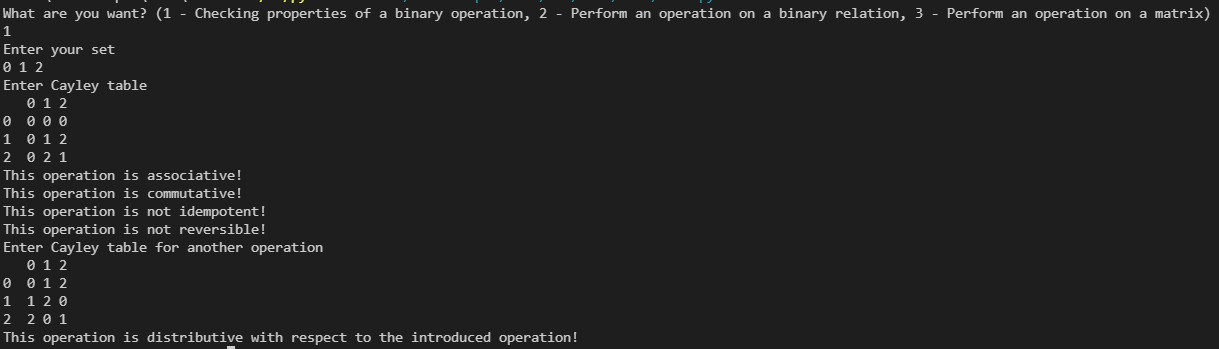
\includegraphics[width=1.\textwidth]{1}
    \caption{Тест алгоритма проверки свойств операций}
    \label{fig:image1}
\end{figure}

\begin{figure}[H]
    \centering      %размер рисунка       здесь находится название файла рисунка, без указания формата
    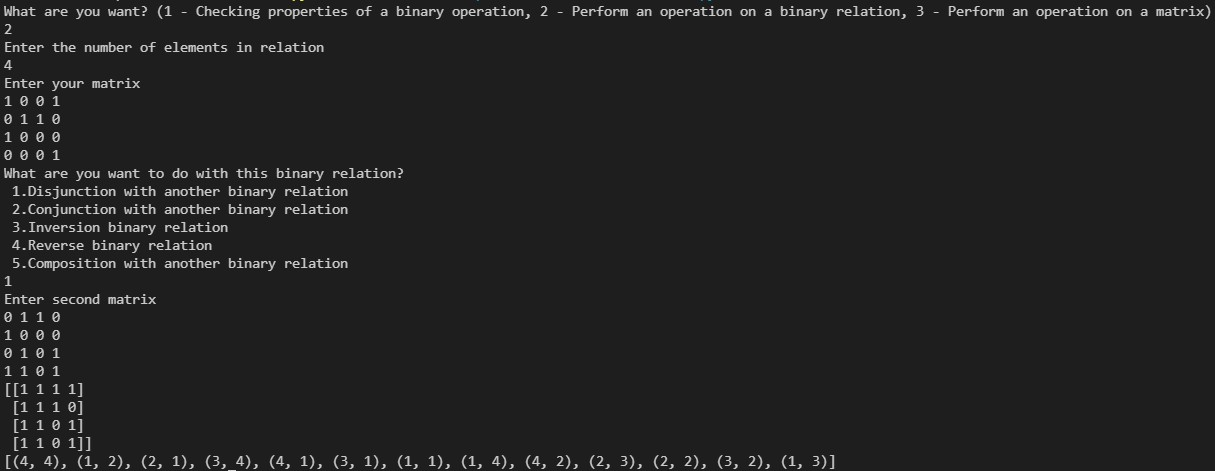
\includegraphics[width=1.\textwidth]{2}
    \caption{Тест алгоритма объединения бинарных отношений}
    \label{fig:image1}
\end{figure}

\begin{figure}[H]
    \centering      %размер рисунка       здесь находится название файла рисунка, без указания формата
    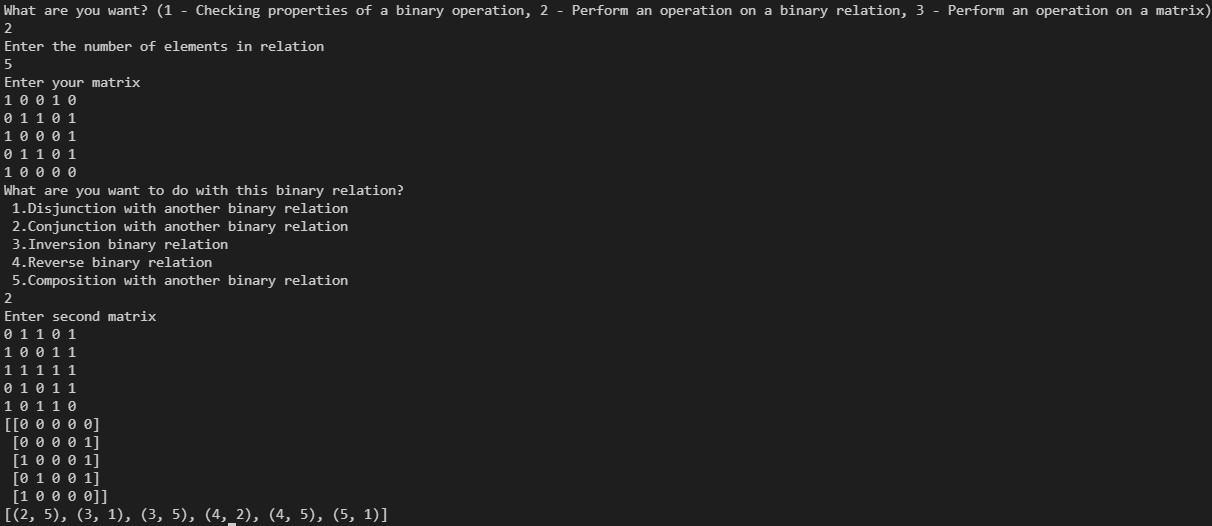
\includegraphics[width=1.\textwidth]{3}
    \caption{Тест алгоритма пересечения бинарных отношений}
    \label{fig:image1}
\end{figure}

\begin{figure}[H]
    \centering      %размер рисунка       здесь находится название файла рисунка, без указания формата
    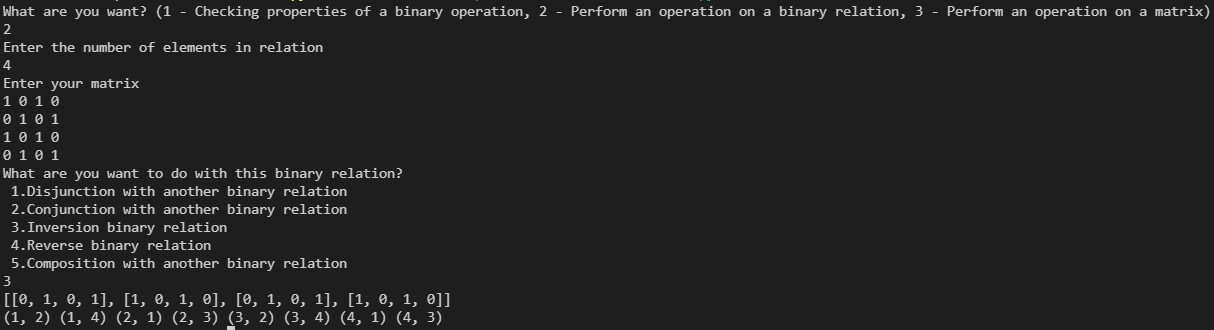
\includegraphics[width=1.\textwidth]{4}
    \caption{Тест алгоритма инверсии бинарных отношений}
    \label{fig:image1}
\end{figure}

\begin{figure}[H]
    \centering      %размер рисунка       здесь находится название файла рисунка, без указания формата
    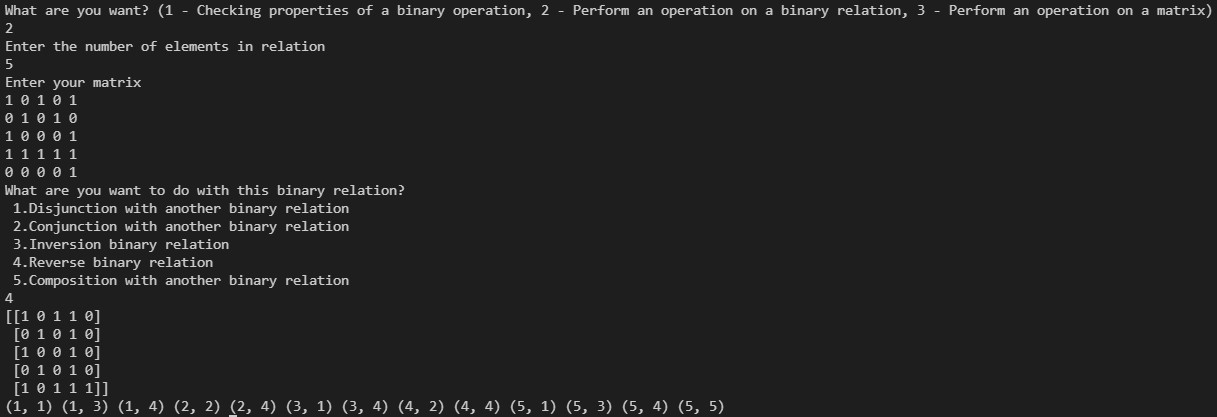
\includegraphics[width=1.\textwidth]{5}
    \caption{Тест алгоритма обращения бинарных отношений}
    \label{fig:image1}
\end{figure}

\begin{figure}[H]
    \centering      %размер рисунка       здесь находится название файла рисунка, без указания формата
    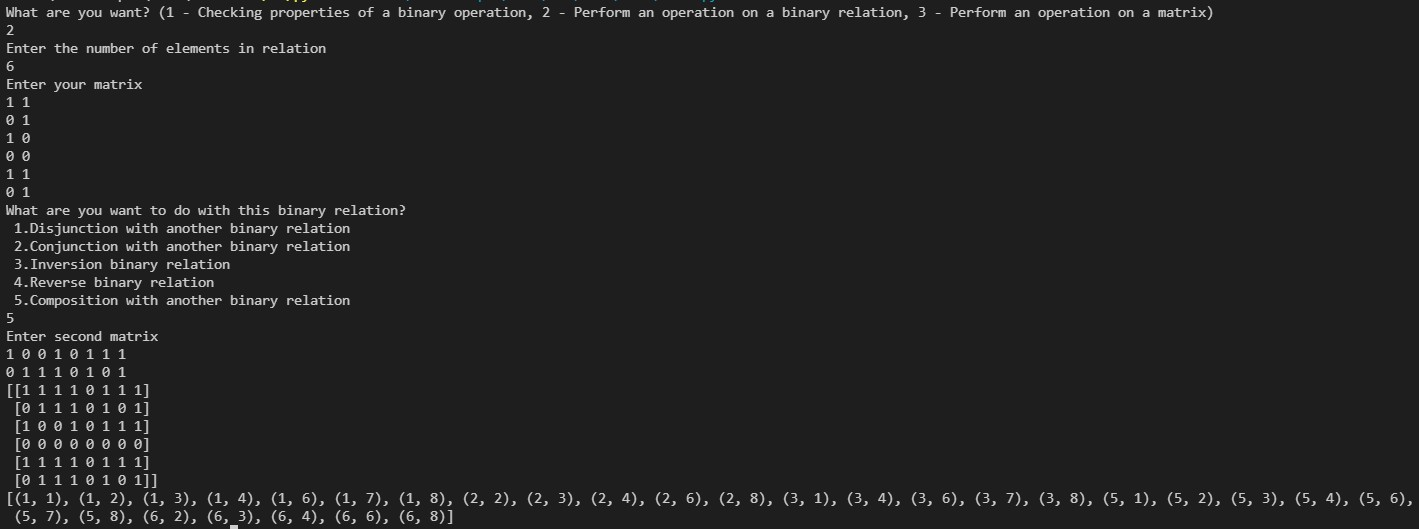
\includegraphics[width=1.\textwidth]{6}
    \caption{Тест алгоритма композиции бинарных отношений}
    \label{fig:image1}
\end{figure}

\begin{figure}[H]
    \centering      %размер рисунка       здесь находится название файла рисунка, без указания формата
    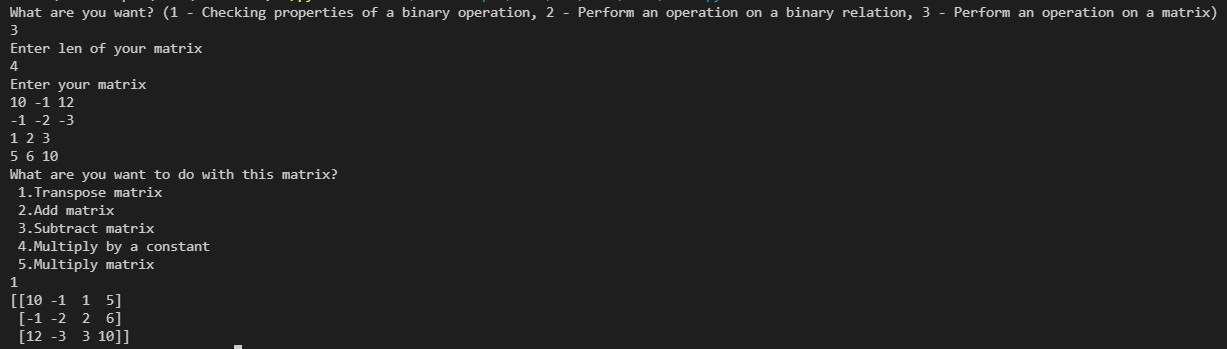
\includegraphics[width=1.\textwidth]{7}
    \caption{Тест алгоритма транспонирования матриц}
    \label{fig:image1}
\end{figure}

\begin{figure}[H]
    \centering      %размер рисунка       здесь находится название файла рисунка, без указания формата
    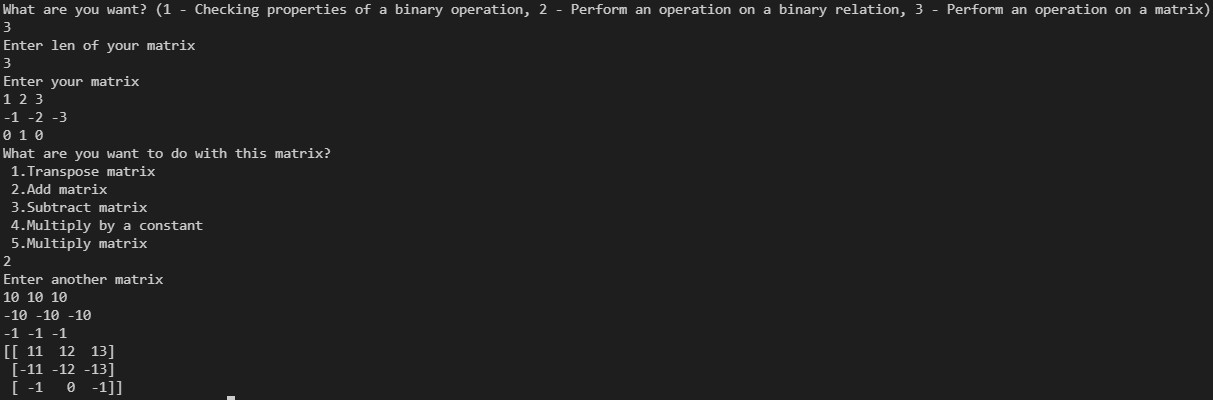
\includegraphics[width=1.\textwidth]{8}
    \caption{Тест алгоритма сложения матриц}
    \label{fig:image1}
\end{figure}

\begin{figure}[H]
    \centering      %размер рисунка       здесь находится название файла рисунка, без указания формата
    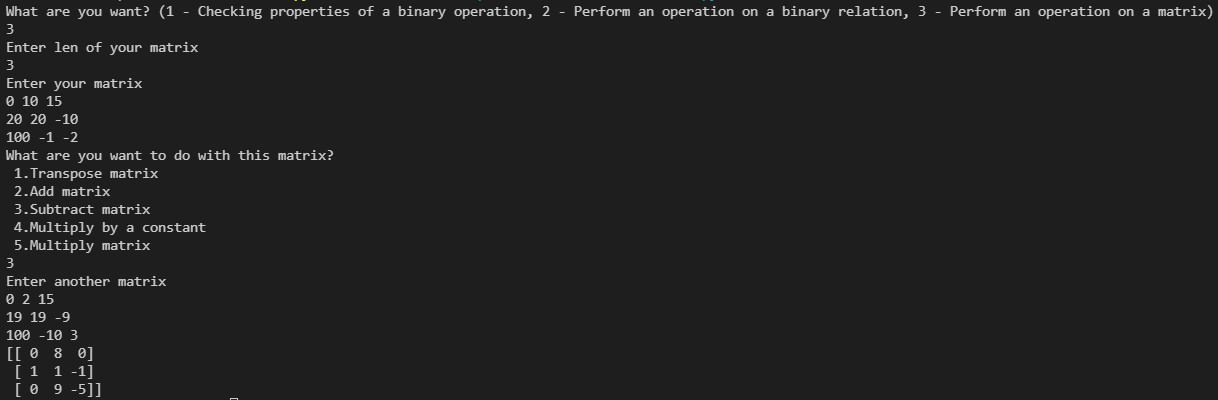
\includegraphics[width=1.\textwidth]{9}
    \caption{Тест алгоритма вычитания матриц}
    \label{fig:image1}
\end{figure}

\begin{figure}[H]
    \centering      %размер рисунка       здесь находится название файла рисунка, без указания формата
    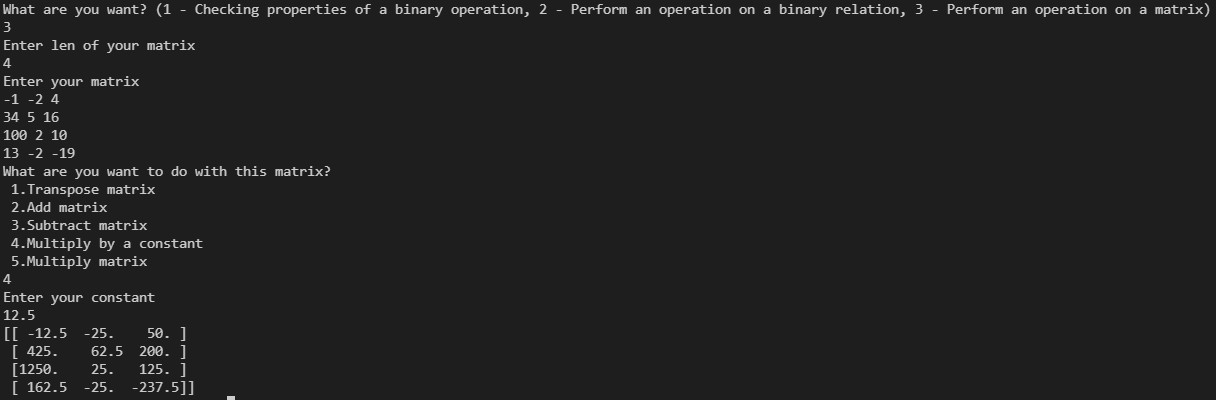
\includegraphics[width=1.\textwidth]{10}
    \caption{Тест алгоритма умножение матрицы на костанту}
    \label{fig:image1}
\end{figure}

\begin{figure}[H]
    \centering      %размер рисунка       здесь находится название файла рисунка, без указания формата
    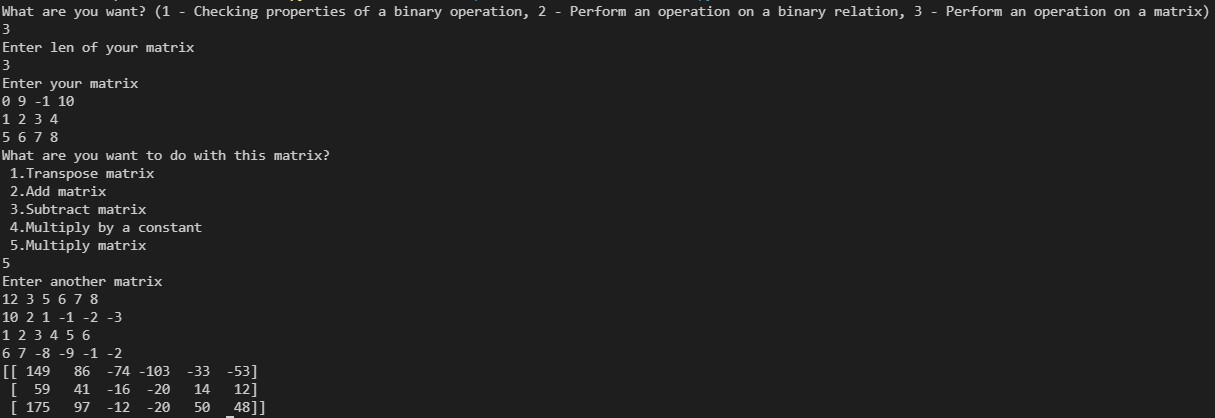
\includegraphics[width=1.\textwidth]{11}
    \caption{Тест алгоритма умножение матриц}
    \label{fig:image1}
\end{figure}

\subsection{Оценки сложности рассмотренных алгоритмов}

    \subsubsection{Проверка операции на ассоциативность}
            Содержит две пары вложенных циклов для генерации двух таблиц Кэли в цикле по n. Следовательно асимптотика данного алгоритма $O(2n^3) = O(n^3)$.

    \subsubsection{Проверка операции на коммутативность}
            С учетом того, что операция транспонирования имеет временную сложность $O(n^2)$ и временной сложности поэлементного сравнения($O(n^2)$), асимптотика алгоритма $O(n^2)$.

    \subsubsection{Проверка операции на идемпотентность}
            В реализации алгоритма был использован один цикл, следовательно его временная сложность определяется как $O(n)$.

    \subsubsection{Проверка операции на обратимость}
            В реализации алгоритма были использован два цикла, один из которых был вложен в другой, следовательно его временная сложность определяется как $O(n^2)$.

    \subsubsection{Проверка операции на дистрибутивность}
            В реализации алгоритма были три вложенных друг в друга цикла, следовательно его временная сложность определяется как $O(n^3)$.

    \subsubsection{Операции объединения бинарных отношений}
            В реализации алгоритма были использован два цикла, один из которых был вложен в другой, для прохода по всем элементам двух матриц, следовательно его временная сложность определяется как $O(n^2)$.

    \subsubsection{Операции пересеченияния бинарных отношений}
            В реализации алгоритма были использован два цикла, один из которых был вложен в другой, для прохода по всем элементам двух матриц, следовательно его временная сложность определяется как $O(n^2)$.
            
    \subsubsection{Операции инверсии бинарного отношений}
            В реализации алгоритма были использован два цикла, один из которых был вложен в другой, для прохода по всем элементам матрицы, следовательно его временная сложность определяется как $O(n^2)$.
    
    \subsubsection{Операции обращения бинарного отношений}
            В реализации алгоритма были использован два цикла, один из которых был вложен в другой, для прохода по всем элементам матрицы, следовательно его временная сложность определяется как $O(n^2)$.
    
    \subsubsection{Операции композиции бинарных отношений}
            В реализации алгоритма были три вложенных друг в друга цикла (один по n, вотро по m, третий по h), следовательно его временная сложность определяется как $O(nmh)$.

    \subsubsection{Операции сложения матриц}
            В реализации алгоритма были использован два цикла, один из которых был вложен в другой, для прохода по всем элементам двух матриц, следовательно его временная сложность определяется как $O(nm)$.

    \subsubsection{Операции вычитания матриц}
            В силу своей схожести с предыдущим алгоритмом временная сложность определяется как $O(nm)$.

    \subsubsection{Операции произведение матрицы на константу}
            В реализации алгоритма были использован два цикла, один из которых был вложен в другой, для прохода по всем элементам матрицы, следовательно его временная сложность определяется как $O(nm)$.

    \subsubsection{Операции транспонирования матрицы}
            В реализации алгоритма были использован два цикла, один из которых был вложен в другой, для прохода по всем элементам матрицы, следовательно его временная сложность определяется как $O(nm)$.

    \subsubsection{Операции произведения матриц}
            В реализации алгоритма были использован два цикла, один из которых был вложен в другой, для прохода по всем элементам первой матрицы, так же внутри вложенного цикла был вложен еще один цикл, 
            с помощью которого считалась сума на i строке первой матрицы и j столбце второй, следовательно его временная сложность определяется как $O(nmh)$.

\subsection{Ответы на задания:}

\begin{figure}[H]
    \centering      %размер рисунка       здесь находится название файла рисунка, без указания формата
    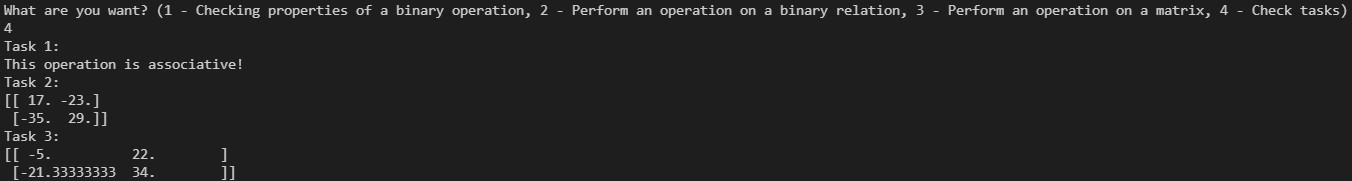
\includegraphics[width=1.\textwidth]{12}
    \caption{Ответы на задания, представленные в конце лабораторной}
    \label{fig:image1}
\end{figure}
    
\conclusion

В рамках данной лабораторной работы были рассмотренны понятие алгебраической операции и классификация ее свойств, основные операции над бинарными отношениями,
основные операции над матрицами. На основе этой теоретической части была смоделирована программа на языке Python с 
использованием средств библиотеки Numpy, которая способна проверки свойства заданной через таблицу Кэли операции, выполнить любую из основных операций над бинарым отношением
или матрицей, а так же была оценена асимптотика каждого реализованного алгоритма.

\end{document}
